% ── Section 3: Methodology ────────────────────────────────────────────────────
\section{Methodology}
\label{sec:methodology}

This section outlines the mathematical and computational architecture of the proposed adaptive procurement framework. We begin by detailing the logical workflow of the four-stage pipeline, followed by the causal data ingestion protocol, the formal Markov Decision Process (MDP) formulation, the baseline decision heuristics, and the Walk-Forward rolling retraining methodology. In this setting, the agent purchases structured electricity derivative blocks (from day-ahead to multi-month maturities) listed on OMIP, modelled as financially-settled futures that hedge financial exposure against spot price volatility while daily margin tracking and mark-to-market settlements are resolved based on official exchange prices.

\subsection{Logical Flow of the Proposed Framework}
\label{subsec:logical_flow}

\begin{figure*}[!t]
    \centering
    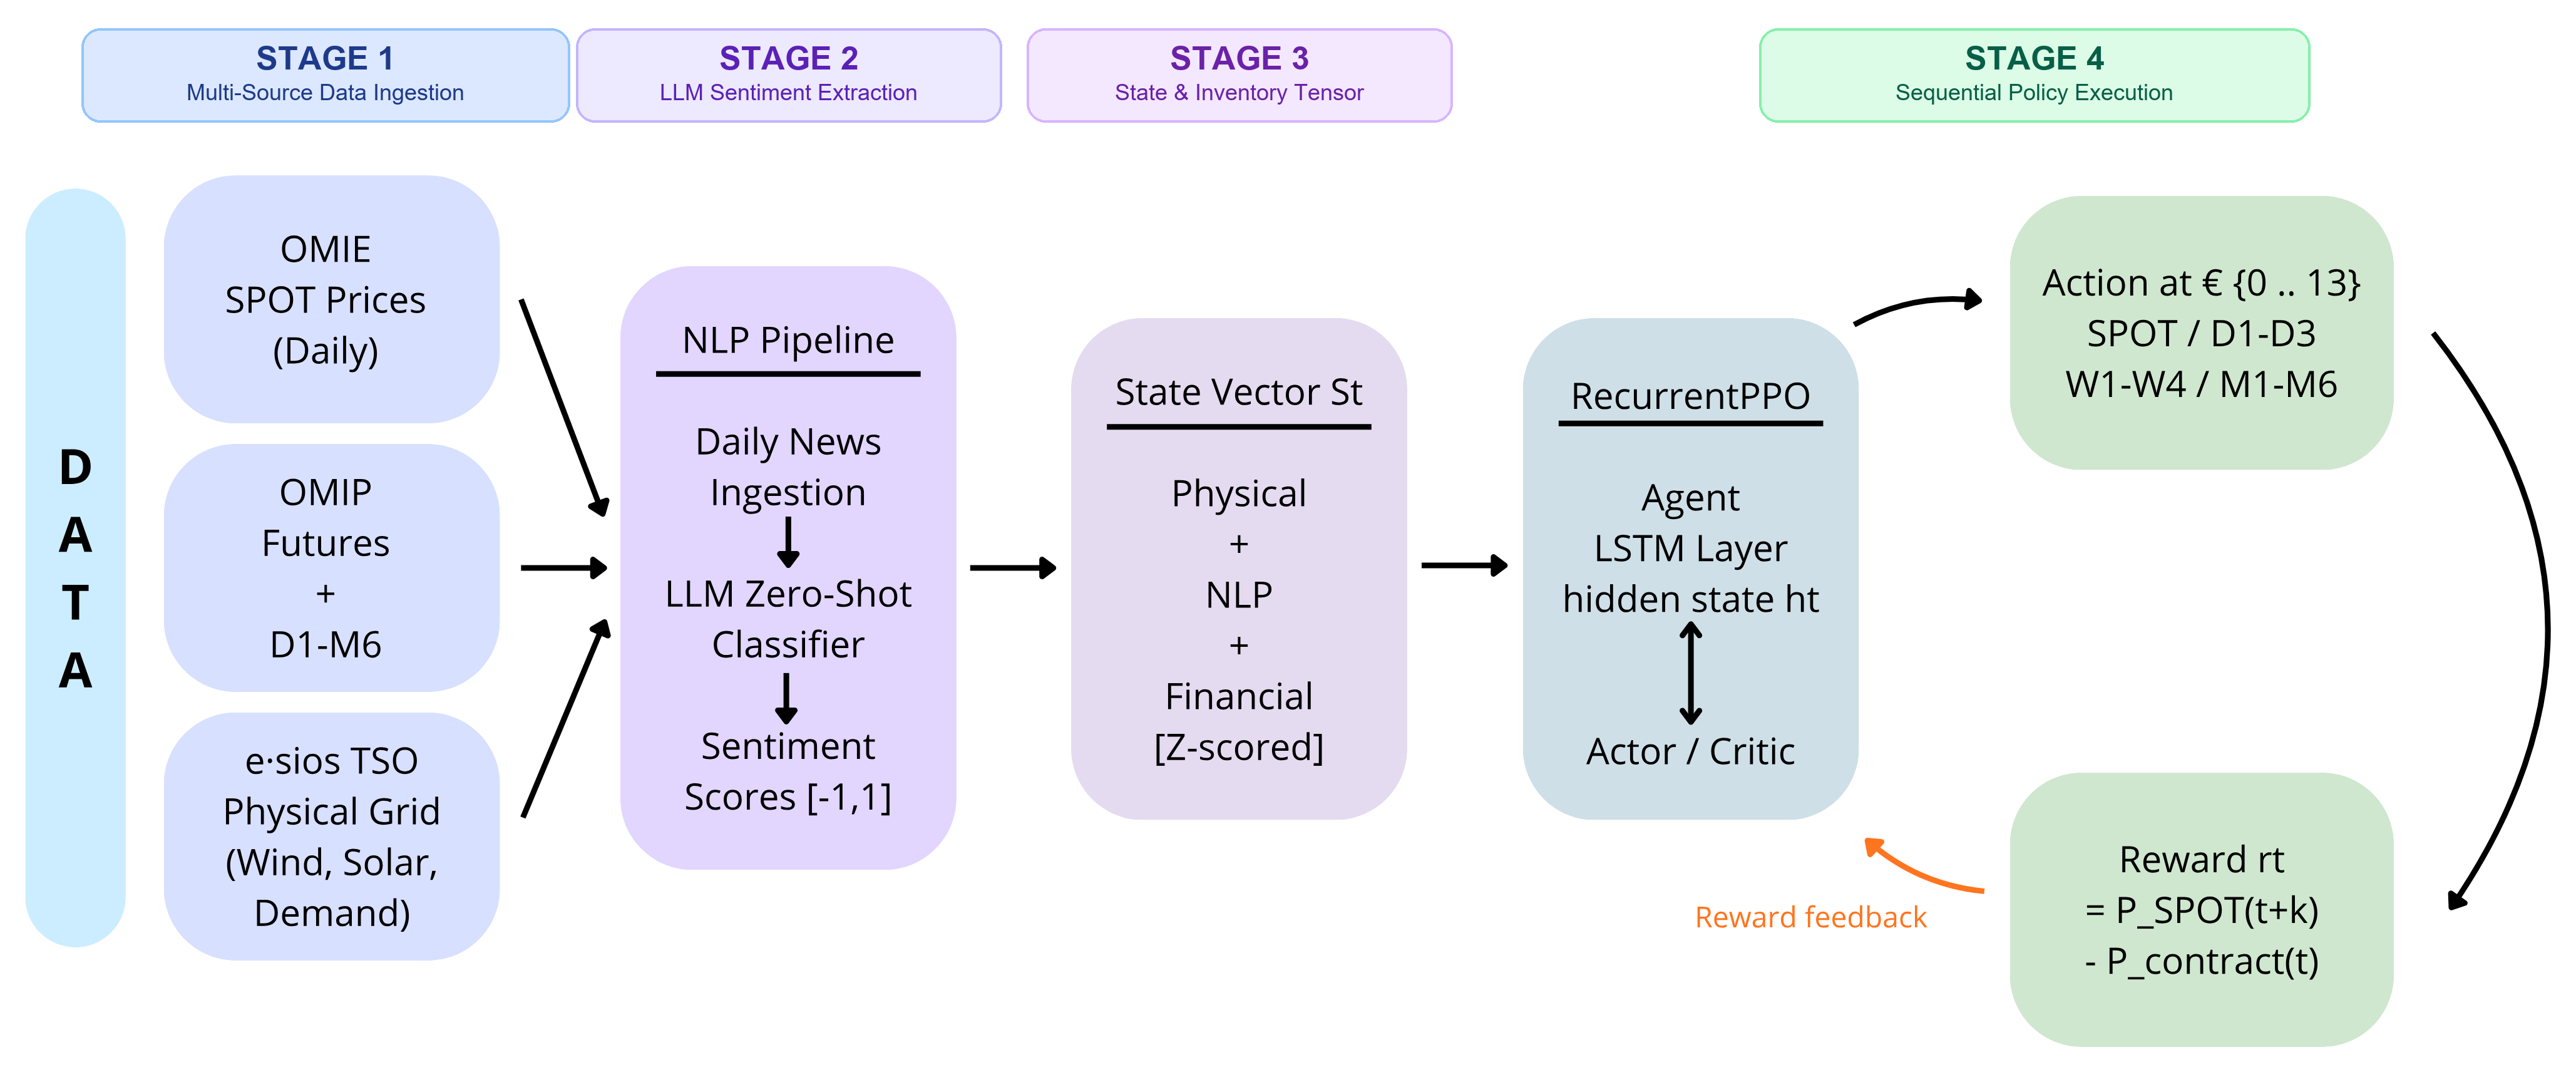
\includegraphics[width=\textwidth]{fig7_system_architecture.png}
    \caption{End-to-end system architecture and operational pipeline of the hybrid DRL and LLM procurement framework across four sequential operational stages.}
    \label{fig:architecture}
\end{figure*}

The methodology developed in this study operates as a continuous, end-to-end pipeline designed to emulate the daily decision-making process of an industrial energy purchasing department. As illustrated in \Cref{fig:architecture}, the logical architecture comprises four sequential operational stages: (1)~\textit{Multi-source data ingestion and synchronization}, where daily physical generation by technology, aggregate electrical demand, and international cross-border transfer capacities from the Transmission System Operator (TSO, Red El\'ectrica de Espa\~na, REE) are merged with daily clearing prices from the market operator (OMIE) and forward settlement curves from the derivatives exchange (OMIP), synchronised strictly at day $t-1$ (23:59~CET); (2)~\textit{Deterministic zero-shot NLP sentiment extraction}, wherein energy and macroeconomic news articles are processed natively using Meta's Llama-3 model under deterministic inference ($T=0.0$, strict JSON schema) to extract 10 domain-specific continuous sentiment scores ($\phi_1, \dots, \phi_{10}$) covering short/medium/long-term outlooks, fuel availability, and regulatory risks; (3)~\textit{Unified state and physical inventory construction}, where the environment constructs a 7-day lookback observation matrix of market features combined with a 400-day forward procurement inventory vector ($\mathbf{c}_t$) with sentinel encoding ($-10.0$ for unhedged delivery slots), tracking forward commitments and delivery coverage; and (4)~\textit{Sequential reinforcement learning execution}, where the deep sequential policy (Recurrent Proximal Policy Optimization, RecurrentPPO, or GTrXL Transformer) observes state vector $\mathbf{o}_t$ and outputs a discrete forward hedging action $a_t \in \{0, \dots, 13\}$, updating physical delivery inventory, executing financial cash flows, and receiving daily unit savings rewards.

\subsection{Data Pipeline and Information Set Timing}
\label{subsec:nlp}

The input space integrates two complementary data streams: a physical/financial market stream and an NLP-derived macroeconomic sentiment stream. To benchmark electricity procurement, the consumption profile is normalised to a continuous unit baseload demand of $E_{\text{load}, d} = 24$~MWh/day per MW of continuous electrical capacity ($1\text{ MW} \times 24\text{ h} = 24\text{ MWh}$). This canonical unit-capacity benchmark represents an industrial consumer schedule whose procurement savings and risk metrics scale linearly to any facility size (e.g., $E_{\text{load}, d} = 4{,}800\text{ MWh/day}$ for a $200$~MW large-scale industrial facility or hyperscale data center \cite{masanet2020recalibrating, iea2024electricity}). Normalizing to unit baseload capacity ensures that the reported results reflect market settlement dynamics without depending on arbitrary enterprise scale, while unit orders of 1~MW represent standard exchange lot sizes that are readily absorbable under normal OMIP order-book liquidity. To evaluate execution robustness, policy sensitivity is tested under hypothetical linear transaction cost levels of 0, 0.10, and 0.25~\texteuro/MWh (Section~\ref{subsec:trans_costs}).

To prevent look-ahead bias and temporal data leakage, the procurement environment is formulated as a daily derivative settlement backtest operating on official clearing and settlement prices from OMIP and OMIClear. The policy selects forward contract commitments using information available through day $t-1$ (23:59~CET); the selected exposure is subsequently valued at the official day-$t$ OMIP closing settlement price $P_{a, t}$. This represents a settlement-valued backtest evaluating settlement-implied procurement efficiency rather than an order-book execution simulation. \Cref{tab:information_set} details the exact source, real-world publication timing, and temporal lag applied to each variable category to ensure causal state construction.

\begin{table*}[!t]
\centering
\footnotesize
\setlength{\tabcolsep}{4pt}
\caption{Information set, sources, publication timing, and temporal lags ensuring causal state construction without look-ahead bias.}
\label{tab:information_set}
\begin{tabularx}{\linewidth}{@{} >{\hsize=1.30\hsize\raggedright\arraybackslash}X
                                  >{\hsize=0.80\hsize\raggedright\arraybackslash}X
                                  >{\hsize=0.95\hsize\raggedright\arraybackslash}X
                                  >{\hsize=0.90\hsize\raggedright\arraybackslash}X
                                  >{\hsize=1.05\hsize\raggedright\arraybackslash}X@{}}
\toprule
\textbf{Variable Category} & \textbf{Data Source} & \textbf{Publication Timing} & \textbf{Decision Step} & \textbf{Applied Lag} \\
\midrule
Physical Generation & TSO (e-sios / REE) & Day $t-1$, 23:59 CET & Day $t$ Trading Step & Lag $t-1$ (Realised) \\
Total Demand \& Interconnection & TSO (e-sios / REE) & Day $t-1$, 23:59 CET & Day $t$ Trading Step & Lag $t-1$ (Realised) \\
Day-Ahead SPOT Price ($P_{\text{SPOT}}$) & OMIE & Day $t-1$, 13:00 CET & Day $t$ Trading Step & Lag $t-1$ (Realised) \\
Forward Derivatives ($P_{a, t-1}$) & OMIP & Day $t-1$, 18:00 CET & Day $t$ Trading Step & Lag $t-1$ (Settlement) \\
Macroeconomic News Sentiment ($\phi$) & Google News / RSS & Day $t-1$, 23:59 CET & Day $t$ Trading Step & Retrospective composite ($t-1$) \\
\bottomrule
\end{tabularx}
\end{table*}

The textual data stream aggregates news from specialized energy and economic media (e.g., \textit{ember-energy.org}, \textit{elEconomista}, \textit{Europa Press}). As illustrated in \Cref{fig:llm_pipeline}, the extraction pipeline processes daily Spanish and international news feeds through a local Ollama instance running Llama-3 8B-Instruct with strict JSON schemas.

\begin{figure*}[!t]
    \centering
    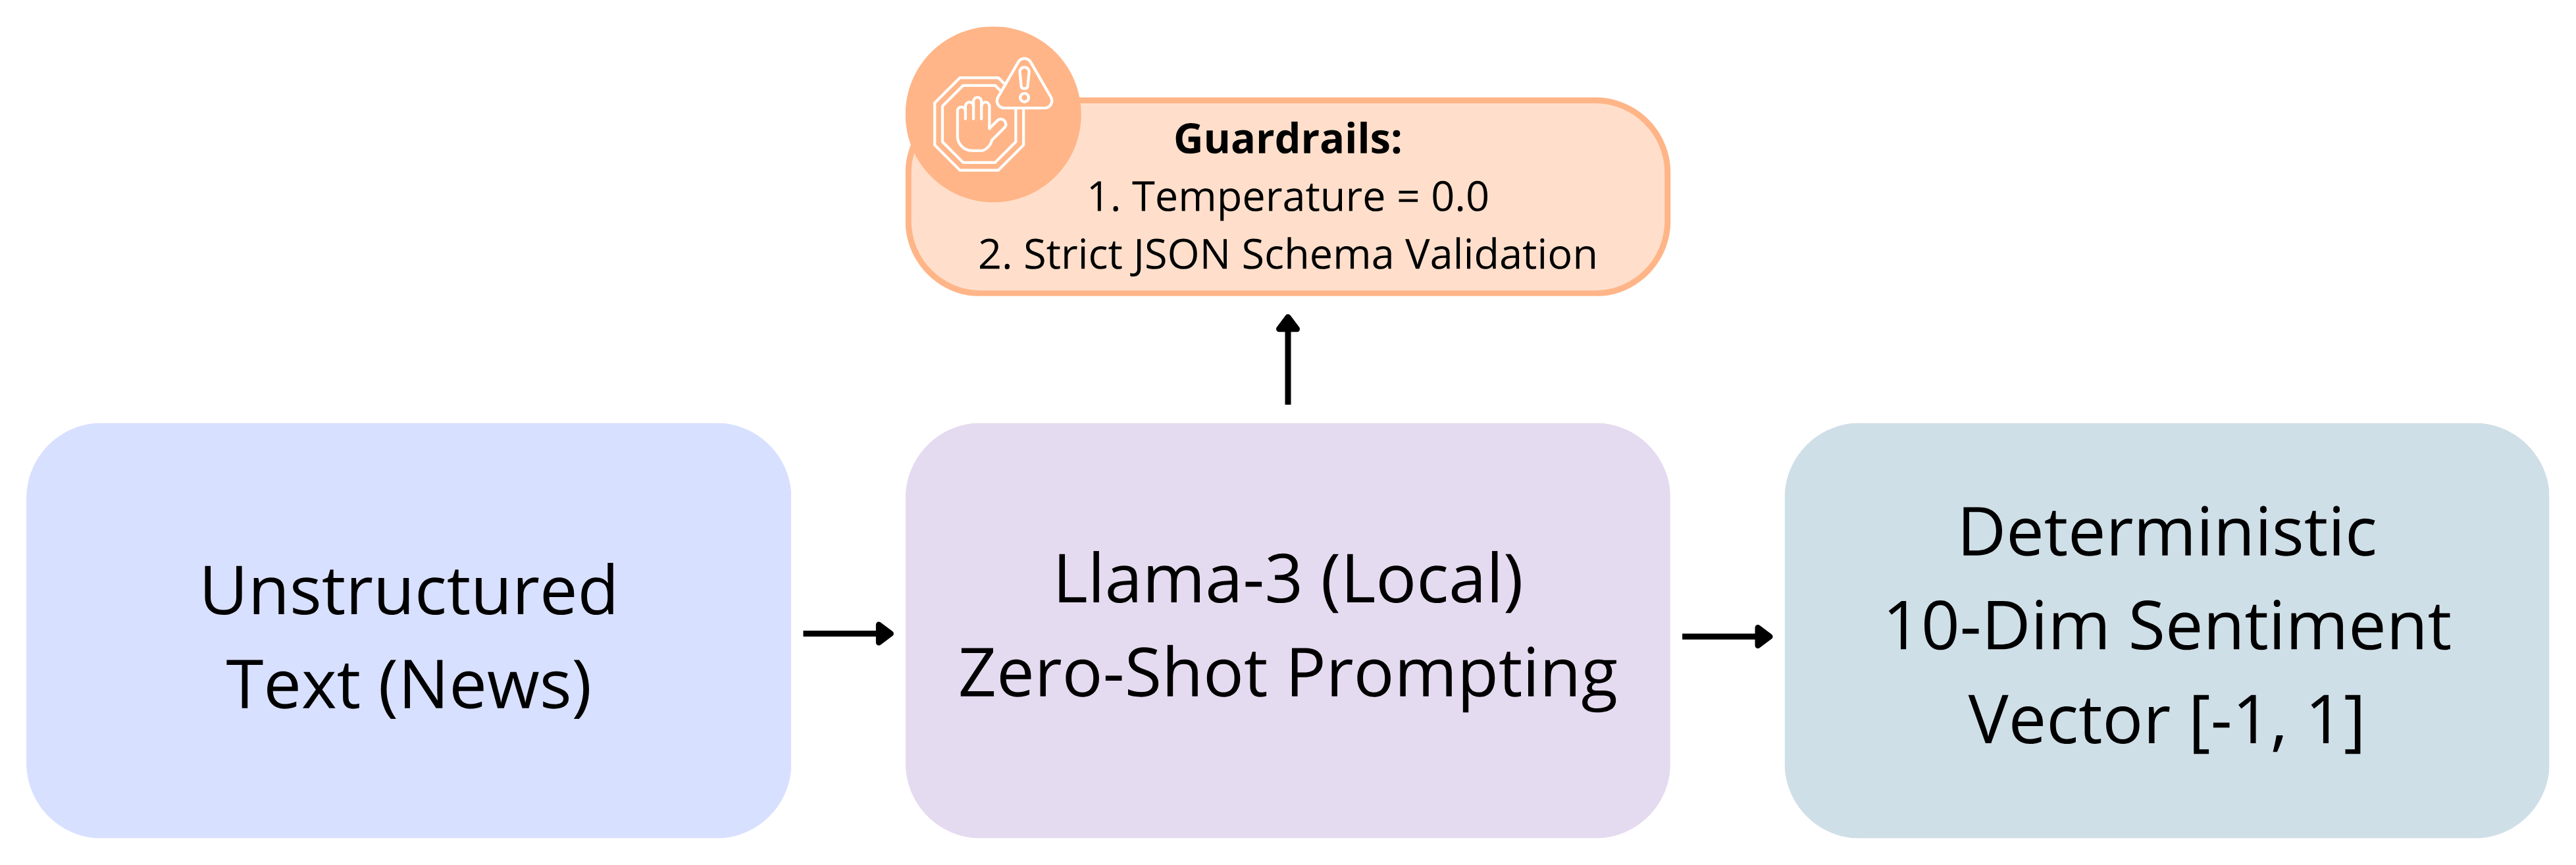
\includegraphics[width=0.70\textwidth]{fig8_llm_pipeline.png}
    \caption{LLM sentiment extraction pipeline with operational guardrails ($T=0.0$ and JSON Schema validation) converting unstructured news into the policy state vector.}
    \label{fig:llm_pipeline}
\end{figure*}

To eliminate consumer-oriented noise, a preliminary zero-shot classification is performed using the Llama-3 model. The filtering prompt instructs the LLM to act as an energy market analyst and strictly discard consumer-oriented news (e.g., residential tariffs), keeping only structural, macroeconomic, or geopolitical news.
The approved articles are then processed by a local Ollama server running the \textit{Llama-3 8B-Instruct} model (using Q4\_K\_M 4-bit quantisation) for sentiment scoring. To obtain reproducible, machine-readable structured outputs suitable for integration into a continuous DRL pipeline, deterministic decoding under the reported model and software configuration is enforced ($T=0.0$, top-$p = 1.0$, and a strict JSON schema). Using a zero-shot prompt design~\cite{yin2019benchmarking} and a context window of 8,192 tokens, the LLM maps the unstructured text into ten continuous sentiment scores, each normalised to the interval $[-1,+1]$:
$\phi_1$~(short-term market outlook),
$\phi_2$~(medium-term outlook),
$\phi_3$~(long-term outlook),
$\phi_4$~(LLM confidence score),
$\phi_5$~(LNG gas sentiment),
$\phi_6$~(CO\textsubscript{2} ETS sentiment),
$\phi_7$~(MIBEL regulatory impact),
$\phi_8$~(climate and generation mix),
$\phi_9$~(geopolitical risk index), and
$\phi_{10}$~(macroeconomic demand).

Scores are aggregated on a strictly daily, retrospective basis: for any trading day $t$, only news published strictly up to day $t-1$ are processed, using a timestamping scheme designed to avoid look-ahead from the available information set. Numerical features are subsequently normalised via Z-score standardisation computed strictly over the training set.

\subsection{Mathematical Formulation of the Procurement MDP}
\label{subsec:mdp}

We formulate the sequential multi-horizon energy procurement problem through a finite-memory Markov Decision Process (MDP) approximation of an underlying partially observable market process (POMDP)~\cite{puterman1994mdp} defined by the tuple $(\mathcal{S}, \mathcal{A}, \mathcal{O}, \mathcal{P}, \mathcal{R}, \gamma)$. In this formulation, latent macroeconomic, regulatory, and weather dynamics are partially observed through historical lookback windows and zero-shot NLP sentiment indices, mapping underlying environmental states $s_t \in \mathcal{S}$ to compact agent observations $\mathbf{o}_t \in \mathcal{O}$.

To distinguish between environmental information and the inputs supplied to the policy, at each trading day $t$ the underlying environment state $s_t \in \mathcal{S}$ is defined by the historical market matrix, the locked unit price vector, and the binary delivery coverage mask:
\begin{equation}
\begin{aligned}
    s_t = \Big( &\mathbf{X}_t \in \mathbb{R}^{7 \times d_{\text{feat}}},\; \mathbf{c}_t \in \mathbb{R}^{H}, \\
    &\mathbf{m}_t \in \{0, 1\}^{H} \Big)
\end{aligned}
\label{eq:state_space}
\end{equation}
where $\mathbf{X}_t \in \mathbb{R}^{7 \times d_{\text{feat}}}$ represents the 7-day lookback window of all normalised market fundamentals, forward settlement curves, and NLP sentiment variables ($d_{\text{feat}}$ dimensions). The vector $\mathbf{c}_t = [c_t(1), c_t(2), \dots, c_t(H)]^{\top} \in \mathbb{R}^{H}$ records the unnormalized unit procurement prices locked for future delivery dates $t+\delta$ ($\delta \in \{1, \dots, H\}$) over a maximum horizon of $H = 400$~days, while $\mathbf{m}_t \in \{0, 1\}^H$ tracks binary delivery coverage.

To provide a compact representation to the neural policy networks without redundant binary masks, the agent receives the observation vector $\mathbf{o}_t \in \mathbb{R}^{7 d_{\text{feat}} + 400}$:
\begin{equation}
    \mathbf{o}_t = \big[ \text{vec}(\mathbf{X}_t);\, \tilde{\mathbf{c}}_t \big] \in \mathbb{R}^{(7 \times d_{\text{feat}}) + 400}
    \label{eq:observation_vector}
\end{equation}
For \texttt{Dataset\_\allowbreak M8\_\allowbreak Physical\_\allowbreak NLP} ($d_{\text{feat}} = 45$), this yields a 715-dimensional observation vector $\mathbf{o}_t \in \mathbb{R}^{715}$. The vector $\tilde{\mathbf{c}}_t \in \mathbb{R}^H$ is the standardized inventory vector with sentinel encoding:
\begin{equation}
    \tilde{c}_t(\delta) = 
    \begin{cases}
        z\big(c_t(\delta)\big), & \text{if } m_t(\delta) = 1 \\
        -10.0, & \text{if } m_t(\delta) = 0
    \end{cases}
    \label{eq:sentinel_encoding}
\end{equation}
Here, $z(\cdot)$ denotes standard $z$-score normalization based on training distribution statistics (where normalized prices predominantly lie in $[-3.0, +3.0]$). The value $-10.0$ serves strictly as a non-economic sentinel encoding outside the empirical standardized range $[-3.0, +3.0]$, allowing the neural networks to unambiguously differentiate uncommitted forward delivery slots from committed positions without introducing an extra binary mask dimension in the observation space.

The action space $\mathcal{A} = \{a_0, a_1, \dots, a_{13}\}$ comprises 14 discrete actions representing standardized constant-maturity rolling forward products calibrated to daily OMIP closing settlement curves. Rather than trading exchange-listed calendar instruments directly, we construct synthetic constant-maturity products mapped to fixed forward offsets:
\begin{itemize}
    \item $a_0$: Open SPOT procurement (unhedged, physical power purchased at the daily SPOT clearing price).
    \item $a_1, a_2, a_3$: Daily forward contracts ($D_1, D_2, D_3$), with relative delivery offsets $\Delta(a_1) = \{1\}$, $\Delta(a_2) = \{2\}$, and $\Delta(a_3) = \{3\}$.
    \item $a_4, \dots, a_7$: Weekly forward contracts ($W_1, \dots, W_4$), covering calendar weeks $[\delta_{\text{mon}} + 7(k-4),\, \delta_{\text{mon}} + 7(k-4) + 6]$ for $k \in \{4, 5, 6, 7\}$, with $\delta_{\text{mon}}$ days to next Monday.
    \item $a_8, \dots, a_{13}$: Monthly forward contracts ($M_1, \dots, M_6$), covering target month $m = \text{month}(t) + (k-7)$ over delivery offset range $\Delta(a_k)$.
\end{itemize}
Weekend and market holiday delivery slots inherit the forward delivery commitments locked during previous active trading sessions; unhedged weekend slots settle at the official OMIE weekend SPOT clearing price. Because OMIE physical spot clearing operates 365 days a year while OMIP derivative trading operates exclusively on official exchange business days ($\approx 252$ days/year, closing on weekends and TARGET2/OMIP bank holidays), non-trading days are handled via a deterministic \texttt{NO\_TRADE} default: no new forward commitments can be initiated, and power delivery is procured at SPOT unless previously covered by a maturing forward contract locked on a prior trading session. When a forward contract has no active quotation on an exchange session, or when selecting it would violate non-overlapping baseload delivery constraints ($\sum_{\delta \in \Delta(a)} m_t(\delta) > 0$), the action is flagged as invalid and incurs the penalty $\lambda_{\text{pen}}$, preserving strict operational validity across all contract horizons ($D_1$--$M_6$).

Each forward contract $a \in \mathcal{A} \setminus \{a_0\}$ selected at trading day $t$ is valued at the official OMIP daily closing settlement price $P_{a, t}$ for that day, whereas input state features condition exclusively on information available up to day $t-1$ (23:59~CET). The position sizing maps each action to a continuous 100\% base-load volume hedge ($E_{\text{load}, d} = 24$~MWh/day per MW of continuous baseload capacity).

The environmental state transitions and forward hedging commitments unfold sequentially. Upon selecting action $a_t$ at day $t$, action validity is verified against existing inventory: the action is valid if no covered day overlaps ($\sum_{\delta \in \Delta(a_t)} m_t(\delta) = 0$) and the quoted price $P_{a_t, t}$ is valid. If valid, the intermediate post-action inventory vector $\mathbf{c}_t^+$ and mask $\mathbf{m}_t^+$ are updated:
\begin{equation}
\begin{aligned}
    c_t^+(\delta) &= 
    \begin{cases}
        P_{a_t, t}, & \text{if } \delta \in \Delta(a_t) \\
        c_t(\delta), & \text{otherwise}
    \end{cases}, \\
    m_t^+(\delta) &= 
    \begin{cases}
        1, & \text{if } \delta \in \Delta(a_t) \\
        m_t(\delta), & \text{otherwise}
    \end{cases}
    \qquad \forall\,\delta \in \{1, \dots, H\}
\end{aligned}
\label{eq:inventory_update}
\end{equation}
If invalid, the position vector remains unchanged ($\mathbf{c}_t^+ = \mathbf{c}_t$, $\mathbf{m}_t^+ = \mathbf{m}_t$) and an invalid penalty indicator $\mathbb{I}_{\text{invalid}}(a_t) = 1$ is triggered. Using an internal penalty in the reward function rather than hard action masking maintains continuous, unconstrained policy gradient estimation across the full 14-dimensional action space during PPO optimization, allowing the policy to smoothly learn feasible operational boundaries.

When advancing from day $t$ to day $t+1$:
\begin{enumerate}
    \item \textbf{Settlement of Delivery Day $t+1$:} The position $c_t^+(1)$ (with mask $m_t^+(1)$) matures. The effective unit procurement cost $P_{\text{eff}, t+1}$ realised for delivery day $t+1$ is:
    \begin{equation}
        P_{\text{eff}, t+1} = m_t^+(1) \cdot c_t^+(1) + \big(1 - m_t^+(1)\big) \cdot P_{\text{SPOT}, t+1}
        \label{eq:effective_cost}
    \end{equation}
    \item \textbf{Inventory Shift Transition:} The remaining forward commitments shift by one calendar day into state $s_{t+1}$:
    \begin{equation}
    \begin{aligned}
        c_{t+1}(\delta) &= c_t^+(\delta + 1), \\
        m_{t+1}(\delta) &= m_t^+(\delta + 1), \quad \forall\,\delta \in \{1, \dots, H-1\}
    \end{aligned}
    \label{eq:inventory_shift}
    \end{equation}
    with boundary condition $c_{t+1}(H) = -10.0, m_{t+1}(H) = 0$.
\end{enumerate}

Table~\ref{tab:action_settlement_mapping} summarizes the execution and settlement mapping across contract types, confirming consistent temporal indexing. For weekly contracts $W_k$ ($k \in \{1, 2, 3, 4\}$), let $\text{wd}(t) \in \{0, \dots, 6\}$ denote the weekday of trading session $t$ ($0 = \text{Monday}$). The delivery window covers the target Monday-to-Sunday calendar week:
\begin{align}
    \delta_{\text{start}}(W_k, t) &= d_{\text{next\_Mon}}(t) + 7(k-1) \\
    \delta_{\text{end}}(W_k, t) &= \delta_{\text{start}}(W_k, t) + 6
\end{align}
where $d_{\text{next\_Mon}}(t) = 7 - \text{wd}(t)$ (or 7 if $\text{wd}(t)=0$). For monthly contracts $M_k$ ($k \in \{1, \dots, 6\}$), the delivery window spans the full calendar month starting on the 1st of month $m_t + k$ and ending on its last day. 

To prevent terminal truncation bias near dataset boundaries, the environment verifies that each contract's delivery window falls strictly within the historical series and inventory bounds ($0 \le \delta_{\text{start}}$ and $t + \delta_{\text{end}} \le T_{\text{dataset}}, \delta_{\text{end}} < H$). Any action whose delivery extends beyond available market records is masked as an invalid decision ($\lambda_{\text{pen}} = 1.0$~\texteuro/MWh penalty) and defaults to SPOT clearing.

\begin{table*}[!t]
\centering
\footnotesize
\setlength{\tabcolsep}{4pt}
\caption{Action execution, delivery window offsets, state entry, and settlement timing mapping.}
\label{tab:action_settlement_mapping}
\begin{tabularx}{\linewidth}{@{} >{\hsize=0.65\hsize\raggedright\arraybackslash}X
                                  >{\hsize=1.15\hsize\raggedright\arraybackslash}X
                                  >{\hsize=1.20\hsize\raggedright\arraybackslash}X
                                  >{\hsize=0.95\hsize\raggedright\arraybackslash}X
                                  >{\hsize=1.05\hsize\raggedright\arraybackslash}X@{}}
\toprule
\textbf{Action ($a_t$)} & \textbf{Delivery Window ($\tau$)} & \textbf{Delivery Offsets $[\delta_s, \delta_e]$} & \textbf{Settlement Day} & \textbf{Effective Cost Realised} \\
\midrule
SPOT ($a_0$) & $t+1$ & Unhedged ($m_t^+(1) = 0$) & $t+1$ & $P_{\text{eff}, t+1} = P_{\text{SPOT}, t+1}$ \\
$D_1$ ($a_1$) & $t+1$ & $[1, 1]$ & $t+1$ & $P_{\text{eff}, t+1} = P_{D_1, t}$ \\
$D_2$ ($a_2$) & $t+2$ & $[2, 2]$ & $t+2$ & $P_{\text{eff}, t+2} = P_{D_2, t}$ \\
$D_3$ ($a_3$) & $t+3$ & $[3, 3]$ & $t+3$ & $P_{\text{eff}, t+3} = P_{D_3, t}$ \\
$W_k$ ($a_4$--$a_7$) & Next $k$-th Mon--Sun week & $[d_{\text{Mon}}+7(k-1),\, d_{\text{Mon}}+7k-1]$ & $\tau \in [t+\delta_s, t+\delta_e]$ & $P_{\text{eff}, \tau} = P_{W_k, t}$ \\
$M_k$ ($a_8$--$a_{13}$) & Target calendar month $(m_t+k)$ & $[d_{\text{1st}},\, d_{\text{last}}]$ & $\tau \in [t+\delta_s, t+\delta_e]$ & $P_{\text{eff}, \tau} = P_{M_k, t}$ \\
\bottomrule
\end{tabularx}
\end{table*}

In European wholesale power markets, derivatives listed on OMIP (such as SPEL Baseload Futures) are financially-settled derivative contracts cleared through OMIClear. In accordance with the OMIClear Clearing Rulebook~\cite{omiclear2023rulebook}, the cash flows of a buy forward position entered on trading day $t$ at quote $F_{t, \text{prod}} = P_{a_t, t}$ covering delivery period $\mathcal{D}_{\text{prod}}$ (with total contract volume $Q_{\text{prod}} = q \cdot |\mathcal{D}_{\text{prod}}|$, where $q = 24$~MWh/day represents the daily baseload volume per MW of continuous capacity) are resolved in two formal stages:
\begin{enumerate}
    \item \textbf{Trading Stage (up to Last Trading Day, $\text{LTD}$):} Daily mark-to-market variation margins accumulate across the total contract volume from entry day $t$ to the contract's last trading day $\text{LTD}$:
    \begin{equation}
    \begin{aligned}
        \text{CF}_{\text{total}} &= \sum_{k=t+1}^{\text{LTD}} \big( F_{k, \text{prod}} - F_{k-1, \text{prod}} \big) \cdot Q_{\text{prod}} \\
        &= \big( F_{\text{LTD}, \text{prod}} - F_{t, \text{prod}} \big) \cdot Q_{\text{prod}}
    \end{aligned}
    \label{eq:cfd_trading_stage}
    \end{equation}
    where $F_{\text{LTD}, \text{prod}}$ is the final closing settlement price on the last trading session prior to physical delivery. Amortising this gain evenly across the $|\mathcal{D}_{\text{prod}}|$ delivery days yields a daily margin cash flow $\text{CF}_{\text{margin}, d}$:
    \begin{equation}
    \begin{aligned}
        \text{CF}_{\text{margin}, d} &= \frac{1}{|\mathcal{D}_{\text{prod}}|} \big( F_{\text{LTD}, \text{prod}} - F_{t, \text{prod}} \big) \cdot Q_{\text{prod}} \\
        &= \big( F_{\text{LTD}, \text{prod}} - F_{t, \text{prod}} \big) \cdot q
    \end{aligned}
    \label{eq:cfd_daily_margin}
    \end{equation}
    \item \textbf{Delivery Stage (Delivery Settlement Value, $\text{DSV}$):} During each delivery day $d \in \mathcal{D}_{\text{prod}}$, OMIClear calculates the daily financial Delivery Settlement Value for volume $q$ based on the difference between the daily OMIE Spot Reference Price $P_{\text{SPOT}, d}$ and the final futures settlement price $F_{\text{LTD}, \text{prod}}$:
    \begin{equation}
        \text{DSV}_d = \big( P_{\text{SPOT}, d} - F_{\text{LTD}, \text{prod}} \big) \cdot q
        \label{eq:cfd_delivery_stage}
    \end{equation}
    \item \textbf{Physical Spot Procurement in OMIE:} The consumer procures its required continuous baseload energy $q = 24$~MWh in the physical day-ahead market (OMIE) at spot clearing cost $-P_{\text{SPOT}, d} \cdot q$.
\end{enumerate}
Summing the amortised trading-stage variation margin $\text{CF}_{\text{margin}, d}$, the daily delivery settlement value $\text{DSV}_d$, and the physical OMIE spot payment yields the total net procurement cash outflow $\text{CF}_{\text{net}, d}$ for each delivery day $d \in \mathcal{D}_{\text{prod}}$:
\begin{equation}
\begin{aligned}
    \text{CF}_{\text{net}, d} &= - P_{\text{SPOT}, d} \cdot q + \text{DSV}_d + \text{CF}_{\text{margin}, d} \\
    &= - P_{\text{SPOT}, d} \cdot q + \big( P_{\text{SPOT}, d} - F_{\text{LTD}, \text{prod}} \big) \cdot q \\
    &\quad + \big( F_{\text{LTD}, \text{prod}} - F_{t, \text{prod}} \big) \cdot q \\
    &= - F_{t, \text{prod}} \cdot q = - P_{a_t, t} \cdot q
\end{aligned}
\label{eq:net_cashflow}
\end{equation}
Dividing by daily baseload volume $q$ yields the effective unit supply cost $P_{\text{eff}, d} = F_{t, \text{prod}} = P_{a_t, t}$, which is scale-invariant. Under standard frictionless market assumptions (zero execution fees, zero bid-ask half-spreads, and frictionless collateral financing), financial derivative hedging is algebraically identical to locking the unit supply cost at the forward quote $P_{a_t, t}$.

The MDP reward function $\mathcal{R}$ guides sequential policy optimization by measuring unit savings on the immediate settlement day relative to the unhedged SPOT benchmark:
\begin{equation}
    r_t = \big( P_{\text{SPOT}, t+1} - P_{\text{eff}, t+1} \big) - R_{\text{penalty}} \cdot \mathbb{I}_{\text{invalid}}(a_t)
    \label{eq:reward_formal}
\end{equation}
where $R_{\text{penalty}} = 20.0$~\texteuro/MWh is an internal MDP optimization penalty applied during policy training whenever the agent selects an invalid action (e.g., attempting to purchase a contract on an unavailable trading day, or selecting an action whose forward delivery window overlaps already committed inventory in $\mathbf{m}_t$). When an invalid action occurs, the order is rejected without state update, the consumer default clears that day's physical demand at the actual day-ahead spot price ($P_{\text{eff}, t+1} = P_{\text{SPOT}, t+1}$), and the reported out-of-sample economic cost accounts strictly for the physical market expenditure ($g_t = 0$), ensuring that training penalties do not distort empirical procurement metrics. An explicit terminal salvage penalty $\lambda_{\text{term}} = 1.0$~\texteuro/MWh is defined for unliquidated positions at the final horizon boundary. The discount factor is set to $\gamma = 0.99$.

Let $g_t = P_{\text{SPOT}, t} - P_{\text{eff}, t}$ denote the daily unit savings (\texteuro/MWh) realised on calendar delivery day $t \in \{1, \dots, T\}$, and let $G_t = \sum_{i=1}^t g_i$ denote the cumulative savings path up to day $t$ (with $G_0 = 0$). Performance and financial risk are evaluated across five formal metrics: Percentage Savings ($S_{\%}$), Cumulative Unit Differential ($S_{\text{cum}}$), Downside Semi-deviation ($\sigma_-$), Conditional Value at Risk ($\text{CVaR}_{0.95}$), and Maximum Drawdown ($\text{Max DD}$):
\begin{align}
    S_{\%} &= \frac{\sum_{t=1}^T g_t}{\sum_{t=1}^T P_{\text{SPOT}, t}} \times 100\% = \frac{\sum_{t=1}^T (P_{\text{SPOT}, t} - P_{\text{eff}, t})}{\sum_{t=1}^T P_{\text{SPOT}, t}} \times 100\% \label{eq:metric_savings_pct} \\
    S_{\text{cum}} &= \sum_{t=1}^T g_t \quad [\text{\texteuro/MWh}] \label{eq:metric_savings_cum} \\
    \sigma_- &= \sqrt{\frac{1}{T} \sum_{t=1}^T \big(\min(g_t, 0)\big)^2} \quad [\text{\texteuro/MWh}] \label{eq:metric_semidev} \\
    \text{CVaR}_{0.95} &= \frac{1}{\lfloor 0.05 \cdot T \rfloor} \sum_{k=1}^{\lfloor 0.05 \cdot T \rfloor} g_{(k)} \quad [\text{\texteuro/MWh}] \label{eq:metric_cvar} \\
    \text{Max DD} &= \max_{1 \le t \le T} \left( \max_{1 \le u \le t} G_u - G_t \right) \quad [\text{\texteuro/MWh}] \label{eq:metric_maxdd}
\end{align}
where $g_{(1)} \le g_{(2)} \le \dots \le g_{(T)}$ represent the ascending order statistics of daily unit savings $g_t$. For multi-year Walk-Forward evaluations across the 40 test blocks ($T = D_{\text{eval}} = 374$ evaluated days), aggregate percentage savings represent an expenditure-weighted average across annual sub-horizons: $S_{\%, \text{agg}} = \sum_y w_y S_{\%, y}$, where weights $w_y = \sum_{t \in y} P_{\text{SPOT}, t} / \sum_{t=1}^T P_{\text{SPOT}, t}$ reflect time-varying wholesale spot prices ($w_{2023} \approx 37.6\%$, $w_{2024} \approx 29.3\%$, $w_{2025} \approx 26.6\%$, and $w_{2026} \approx 6.5\%$), yielding $+6.04\%$ multi-year savings ($\sum g_t / \sum P_{\text{SPOT}} = 1{,}486.39 / 24{,}595.50$), with average daily unit savings of $3.97$~\texteuro/MWh over the 374 evaluated days (where mean evaluated spot price was $65.76$~\texteuro/MWh; $3.974 / 65.763 = 6.04\%$), distinct from the broader 1,242-day multi-year spot average of $55.40$~\texteuro/MWh. Under this convention, $\text{CVaR}_{0.95}$ measures the lower-tail Expected Shortfall at 5\% on savings (where negative values represent expected unit deficits in the worst 5\% tail), and $\text{Max DD}$ quantifies the peak-to-trough decline of the cumulative savings trajectory ($0.00$~\texteuro/MWh for Pure SPOT as $g_t \equiv 0$). Total monetary savings scale as $S_{\text{cum}} \times q$~\texteuro/MW.

To evaluate sequential decision-making under partial observability, we compare two distinct policy architectures operating on observation vectors $\mathbf{o}_t$:
\begin{enumerate}
    \item \textbf{RecurrentPPO (LSTM):} Single-layer LSTM ($d_h = 256$ in baseline; $d_h = 64$ in Phase 4 tuned) \cite{hochreiter1997lstm, pleines2022recurrentppo} with hidden state update $h_t = \mathrm{LSTM}(\mathbf{o}_t, h_{t-1}; \theta_{\text{LSTM}})$, feeding separate linear Actor and Critic heads.
    \item \textbf{GTrXL Transformer Comparator:} Gated Transformer-XL architecture \cite{parisotto2020gtrxl, vaswani2017attention} comprising $L = 2$ transformer layers, $H = 4$ attention heads, model dimension $d_{\text{model}} = 64$, memory length $M = 14$, GRU-style gating on skip connections, and layer normalisation.
\end{enumerate}
Both architectures are optimized using Proximal Policy Optimization (PPO) \cite{schulman2017ppo} with Generalized Advantage Estimation (GAE, $\lambda = 0.95$, $\gamma = 0.99$):
\begin{equation}
\begin{aligned}
    \mathcal{L}_{\text{PPO}}(\theta) &= -\hat{\mathbb{E}}_t \left[ \min\left( \rho_t(\theta) \hat{A}_t,\; \mathrm{clip}(\rho_t(\theta), 1-\epsilon, 1+\epsilon) \hat{A}_t \right) \right] \\
    &\quad + c_v L_t^V(\theta) - c_{\text{ent}} \mathcal{H}(\pi_\theta(\cdot \mid \mathbf{o}_t, h_{t-1}))
\end{aligned}
\label{eq:ppo_loss}
\end{equation}
where $\rho_t(\theta) = \frac{\pi_\theta(a_t \mid \mathbf{o}_t, h_{t-1})}{\pi_{\theta_{\text{old}}}(a_t \mid \mathbf{o}_t, h_{t-1})}$, clipping range $\epsilon = 0.2$, value loss coefficient $c_v = 0.5$, and entropy coefficient $c_{\text{ent}} = 0.01$ ($0.0239$ in Phase 4). Optimization is performed using Adam ($\beta_1 = 0.9, \beta_2 = 0.999, \epsilon_{\text{Adam}} = 10^{-8}$) with gradient norm clipping at $0.5$, rollout buffer size $n_{\text{steps}} = 128$ ($64$ in Phase 4), mini-batch size $64$ ($16$ in Phase 4), and 10 optimization epochs per update.

\subsection{Empirical Baseline Analysis: Forward Price Differentials}
\label{subsec:d2_anomaly}

Prior to evaluating the DRL policy, we conduct an empirical baseline analysis by systematically purchasing individual forward contracts across the historical timeline. This test highlights the existence of historical price differentials. We document a persistent D2--SPOT price differential in the evaluated sample: the D2 contract (delivery at $t+2$) exhibited an aggregate forward--spot discount relative to the eventual SPOT price. This empirical discount is consistent with horizon-dependent forward risk premia documented in European electricity derivative markets \cite{huisman2012electricity, woo2001cross, huisman2009electricity}, where forward quotations reflect market-specific hedging incentives and asymmetric risk preferences across clearing horizons. While theoretical literature suggests that short-term forward discounts can arise from hedging pressures under short-term generation uncertainty \cite{schwenen2024renewable}, attributing this differential to specific market agents would require order-book and participant-level bid data; here, we treat it strictly as an empirical benchmark property of the evaluated historical market series. 

\begin{table*}[!t]
\centering
\footnotesize
\setlength{\tabcolsep}{2.5pt}
\caption{Passive procurement performance across the evaluated forward-contract horizons (2023--2026), with annual breakdown for the dominant $D_2$ forward baseline.}
\label{tab:systematic_baselines}
\begin{tabularx}{\linewidth}{@{} >{\raggedright\arraybackslash}X >{\centering\arraybackslash}p{1.6cm} rrrrr@{}}
\toprule
\textbf{Contract / Horizon} & \textbf{Eval.\ Days} & \textbf{Win} & \textbf{Mean PnL} & \textbf{Total PnL} & \textbf{Max DD} & \textbf{Savings} \\
 & & \textbf{Rate} & \textbf{(\texteuro/MWh)} & \textbf{(\texteuro/MWh)} & \textbf{(\texteuro/MWh)} & \textbf{(\%)} \\
\midrule
\multicolumn{7}{l}{\textit{Panel A: Multi-Year Forward Contract Comparison (2023--2026)}} \\
D1 & 1,242 & 50.40\% & 1.65 & 2,044 & 316.18 & 2.37\% \\
\textbf{D2 (Multi-Year)} & \textbf{1,218} & \textbf{59.93\%} & \textbf{8.30} & \textbf{10,104} & \textbf{394.18} & \textbf{11.95\%} \\
D3 & 1,198 & 55.59\% & 4.19 & 5,025 & 412.99 & 5.98\% \\
W1 & 1,088 & 46.32\% & $-5.28$ & $-5,740$ & 7,883 & $-7.27\%$ \\
W2 & 1,081 & 51.43\% & 0.32 & 342 & 4,026 & 0.43\% \\
W3 & 1,074 & 49.81\% & $-2.12$ & $-2,272$ & 6,215 & $-2.92\%$ \\
W4 & 1,067 & 45.27\% & $-4.11$ & $-4,386$ & 7,851 & $-5.77\%$ \\
M1 & 1,065 & 48.83\% & $-1.90$ & $-2,021$ & 5,247 & $-2.67\%$ \\
M2 & 1,037 & 41.27\% & $-8.05$ & $-8,345$ & 11,260 & $-11.72\%$ \\
M3 & 1,006 & 42.45\% & $-13.83$ & $-13,914$ & 14,963 & $-20.72\%$ \\
M4 & 976 & 40.78\% & $-20.24$ & $-19,751$ & 19,730 & $-31.61\%$ \\
M5 & 945 & 29.10\% & $-25.48$ & $-24,073$ & 23,983 & $-41.30\%$ \\
M6 & 884 & 27.71\% & $-27.10$ & $-23,958$ & 23,886 & $-44.29\%$ \\
\midrule
\multicolumn{7}{l}{\textit{Panel B: Systematic $D_2$ Forward Baseline Annual Breakdown}} \\
$D_2$ (2023) & 363 & 60.71\% & 8.86 & 3,225 & 284.15 & 10.07\% \\
$D_2$ (2024) & 366 & 62.02\% & 9.02 & 3,301 & 312.40 & 14.13\% \\
$D_2$ (2025) & 365 & 64.11\% & 8.68 & 3,168 & 295.60 & 13.17\% \\
$D_2$ (2026, 148 cal.\ days) & 148 [102] & 56.08\% & 4.94 & 731 & 225.45 & 11.18\% \\
\bottomrule
\end{tabularx}

\bigskip

\caption{Temporal sample accounting across market data sources, operational decision regimes, and experimental evaluation phases (2023--2026).}
\label{tab:sample_accounting}
\setlength{\tabcolsep}{2.5pt}
\begin{tabularx}{\linewidth}{@{} >{\raggedright\arraybackslash}p{2.8cm} >{\centering\arraybackslash}p{2.3cm} ccc >{\raggedright\arraybackslash}X@{}}
\toprule
\textbf{Sample / Scope} & \textbf{Time Horizon} & \textbf{Calendar} & \textbf{Physical} & \textbf{Decision} & \textbf{Operational Specification and Accounting} \\
 & & \textbf{Days} & \textbf{Delivery} & \textbf{Epochs} & \\
\midrule
Full Calendar Timeline & 01/01/23 -- 31/05/26 & 1,247 & 1,247 & --- & Continuous multi-year calendar horizon ($365 + 366 + 365 + 151$ days across 2023, 2024, 2025, and early 2026). \\
Raw OMIE SPOT Clearing & 01/01/23 -- 31/05/26 & 1,247 & 1,247 & 1,247 & Daily marginal pool price clearing across all 1,247 calendar days without operational interruption. \\
OMIP Aligned Evaluation Sample & 03/01/23 -- 30/05/26 & 1,242 & 1,242 & \textbf{1,242} & Retained market delivery sample ($1{,}242$ days) formed by two continuous sampling intervals: $n_1 = 1{,}094$ historical baseline days (03/01/23 -- 31/12/25: 363 in 2023, 366 in 2024, 365 in 2025; excluding 01/01/23 [Sunday] and 02/01/23 [holiday observation]) and $n_2 = 148$ days in 2026 (03/01/26 -- 30/05/26; excluding 01/01/26 [holiday], 02/01/26 [unaligned forward boundary], and 31/05/26 [Sunday boundary]). The inclusive interval 03/01/23--30/05/26 contains exactly 1,242 calendar dates (excluding the 5 boundary dates from the 1,247 raw calendar timeline). Note that naively summing annual calendar counts ($365 + 366 + 365 + 148 = 1{,}244$) includes 01/01/23 and 02/01/23, which are excluded from the evaluated aligned sample. \\
\midrule
Phase 1--2 Validation & 01/01/25 -- 31/12/25 & 365 & 365 & 261 & Static model ablation \& heuristic screening across 365 delivery days: 261 Monday--Friday operational weekday decision epochs (comprising 256 official OMIP trading sessions and 5 weekday TARGET bank holiday closures) and 104 weekend days (totaling 109 non-trading exchange days where default SPOT settlement applies). \\
Phase 3--4 Out-of-Sample & 03/01/26 -- 30/05/26 & 148 & 148 & \textbf{102} (46) & 148 calendar delivery days comprising 102 official OMIP trading sessions (decision epochs where forward contracts can be selected) and 46 non-trading dates (3 weekday TARGET exchange closures [Good Friday, Easter Monday, Labour Day] and 43 weekend days, where passive default SPOT clearing applies). Across non-trading dates, the simulator executes carryover forward settlement or unhedged default SPOT clearing. \\
\midrule
Walk-Forward Evaluation ($W=1$, Monthly Blocks) & 01/02/23 -- 30/05/26 (40 blocks) & 1,215 & 374 & 374 & Exactly 374 evaluated out-of-sample delivery days across the 40 test months (103 in 2023, 114 in 2024, 113 in 2025, and 44 in 2026), evaluating Days 21 to month-end after a 20-day recurrent hidden state warm-up buffer. \\
\bottomrule
\end{tabularx}
\end{table*}

In addition to passive single-contract benchmarks, we formulate an adaptive trend-following benchmark denoted as the \textit{Rolling Adaptive Spread Rule}. On each active trading session $t$, the heuristic evaluates whether the short-dated $D_2$ forward quotation is priced at a favourable spread relative to the trailing $k$-day simple moving average of cleared spot prices $\overline{P}_{\text{SPOT}, t}^{(k)} = \frac{1}{k} \sum_{i=1}^k P_{\text{SPOT}, t-i}$ using an operational lookback window of $k = 14$ days:
\begin{equation}
    a_t = 
    \begin{cases}
        D_2, & \text{if } P_{D_2, t} < \overline{P}_{\text{SPOT}, t}^{(k)} \text{ and } m_t(2) = 0 \\
        \text{SPOT}, & \text{otherwise}
    \end{cases}
    \label{eq:rolling_adaptive_rule}
\end{equation}
If the delivery slot $t+2$ is already hedged ($m_t(2) = 1$) or if the forward quote exceeds trailing spot averages, the heuristic defaults to unhedged spot procurement. This benchmark represents an intuitive trend-following decision heuristic that captures trailing price deflation without requiring neural network training.

A key institutional development during the sample timeline was the market time unit transition of the Iberian day-ahead market (OMIE) on October 1, 2025, from 24 hourly clearing intervals to 96 quarter-hourly Market Time Units (15-minute MTUs) in compliance with European market integration regulations \cite{omie2025mtu, iea2024electricity}. Throughout our multi-year dataset (2023--2026), the daily SPOT price benchmark $P_{\text{SPOT}, t}$ is consistently defined as the official daily arithmetic mean of cleared marginal prices across all settlement intervals of delivery day $t$:
\begin{equation}
    P_{\text{SPOT}, t} = 
    \begin{cases}
        \frac{1}{24} \sum_{h=1}^{24} P_{t, h}, & t < \text{01/10/2025} \\
        \frac{1}{96} \sum_{q=1}^{96} P_{t, q}, & t \ge \text{01/10/2025}
    \end{cases}
    \label{eq:mtu_standardization}
\end{equation}
ensuring complete mathematical and economic continuity across the pre- and post-transition horizons.

\subsection{Training Methodology and Ablation Study Design}
\label{subsec:training}

From a computational standpoint, all experiments, including the continuous Walk-Forward retraining and Bayesian hyperparameter optimisation, were executed on a dedicated Ubuntu server equipped with an Intel Core Ultra 9 285K processor (24 cores), 64 GB of RAM, and an NVIDIA GeForce RTX 5090 (32 GB) GPU. The LLM sentiment extraction was performed locally using Ollama on the same infrastructure to guarantee data privacy, avoid external API version drift, and ensure computational consistency under deterministic settings. The full 5-seed Walk-Forward evaluation across all 4 update windows ($W \in \{1, 3, 6, 12\}$) required approximately 14.5 GPU hours for RecurrentPPO and 22.0 GPU hours for GTrXL. The Bayesian HPO search (50 Optuna trials per architecture) completed in 18.2 hours. For potential operational deployment, daily policy inference would require only a single forward pass through the policy network ($< 4.2$~ms per decision on standard CPU hardware), while computationally intensive training remains restricted to offline execution.

The training and validation of the agent are structured into four sequential phases to ensure complete traceability of data leakage and look-ahead bias:
\begin{itemize}
    \item \textbf{Phases 1 and 2 (Ablation and Heuristics):} Models are trained on 2023--2024 and evaluated on the 2025 horizon. While strictly out-of-sample for weight updates, the 2025 results are used to select the optimal datasets and discard underperforming heuristics. Consequently, 2025 transitions into a \textit{validation set}, carrying selection bias for future phases.
    \item \textbf{Phase 3 (Walk-Forward Baseline):} A continuous rolling window from 2023 to 2026. Because the datasets were selected based on 2025, the 2026 horizon (3 January -- 30 May 2026, comprising 105 weekday decision epochs represented in the simulator [102 official OMIP trading sessions and 3 TARGET bank holiday closures] within 148 calendar delivery days) represents a strictly forward-looking, sequentially out-of-sample evaluation.
    \item \textbf{Phase 4 (Exploratory Architecture and HPO Analysis):} Hyperparameters are optimized using Optuna across the full Walk-Forward evaluation (including 2026) to determine the optimal attainable capacity of each architecture under tuned hyperparameters. Therefore, the final reported results for Phase 4 are explicitly declared as an \textit{exploratory post-selection capacity analysis}, rather than an unbiased out-of-sample test, establishing the comparative performance limits of Recurrence vs Self-Attention under optimal conditions.
\end{itemize}

In Phase~1 (Model and Data Ablation), we construct eight incremental datasets (\textit{Dataset\_Initial} through \textit{Dataset\_M8\_\allowbreak Physical\_NLP}) to isolate the marginal value of NLP and exogenous features. We train two architectural variants, a standard Multi-Layer Perceptron (MLP) and the LSTM-based RecurrentPPO, across all eight datasets. To evaluate the 2025 horizon, each agent is trained exclusively on 2023--2024 data, ensuring a clean one-year forward evaluation without look-ahead bias.

In Phase~2 (Mitigating Degenerate Policies), initial diagnostic evaluations revealed that the LSTM agent tended to suffer from \textit{entropy collapse}, converging to a low-entropy policy focused on the D2 contract due to the penalty associated with long-term inventory overlap and discounting. To test whether broader multi-horizon hedging can be encouraged, three isolated algorithmic adjustments are evaluated on the LSTM model:
\begin{enumerate}
    \item \textit{Entropy increase}: Raising the entropy coefficient ($c_{\text{ent}}$) in the PPO loss function to $0.05$ to increase the entropy regularization term and encourage broader action exploration.
    \item \textit{Diversification bonus}: Modifying the reward function to include a percentage bonus (+5\% for weekly contracts, +10\% for monthly contracts) upon successful execution.
    \item \textit{Soft action replacement}: Instead of applying a large penalty for an invalid overlapping action, the environment gracefully converts the invalid forward purchase into a SPOT purchase and applies a minor symbolic penalty ($-0.5$\texteuro), effectively acting as a soft alternative to action masking.
\end{enumerate}

In Phase~3 (Continuous Walk-Forward Retraining), we evaluate policy adaptation to market shifts on the out-of-sample test horizon (2026). The protocol is illustrated in \cref{fig:walk_forward_protocol} and formally specified in Algorithm~\ref{alg:walk_forward} (\ref{app:walk_forward}). The multi-year timeline (2023--2026) comprises $B = 41$ total monthly calendar blocks $\{M_1, \dots, M_B\}$, yielding $B_{\text{eval}} = B - W$ evaluated out-of-sample monthly blocks (e.g., $B_{\text{eval}} = 40$ evaluated blocks under $W=1$, $B_{\text{eval}} = 38$ under $W=3$, $B_{\text{eval}} = 35$ under $W=6$, and $B_{\text{eval}} = 29$ under $W=12$). For each evaluation block $b \in \{W+1, \dots, B\}$, the policy network is updated over the preceding rolling update window of $W$ calendar months ($W \in \{1, 3, 6, 12\}$ months, corresponding to approximately $20 \times W$ active OMIP trading sessions) and evaluated strictly out-of-sample across the consecutive calendar days of month $M_b$.

\begin{figure*}[!t]
    \centering
    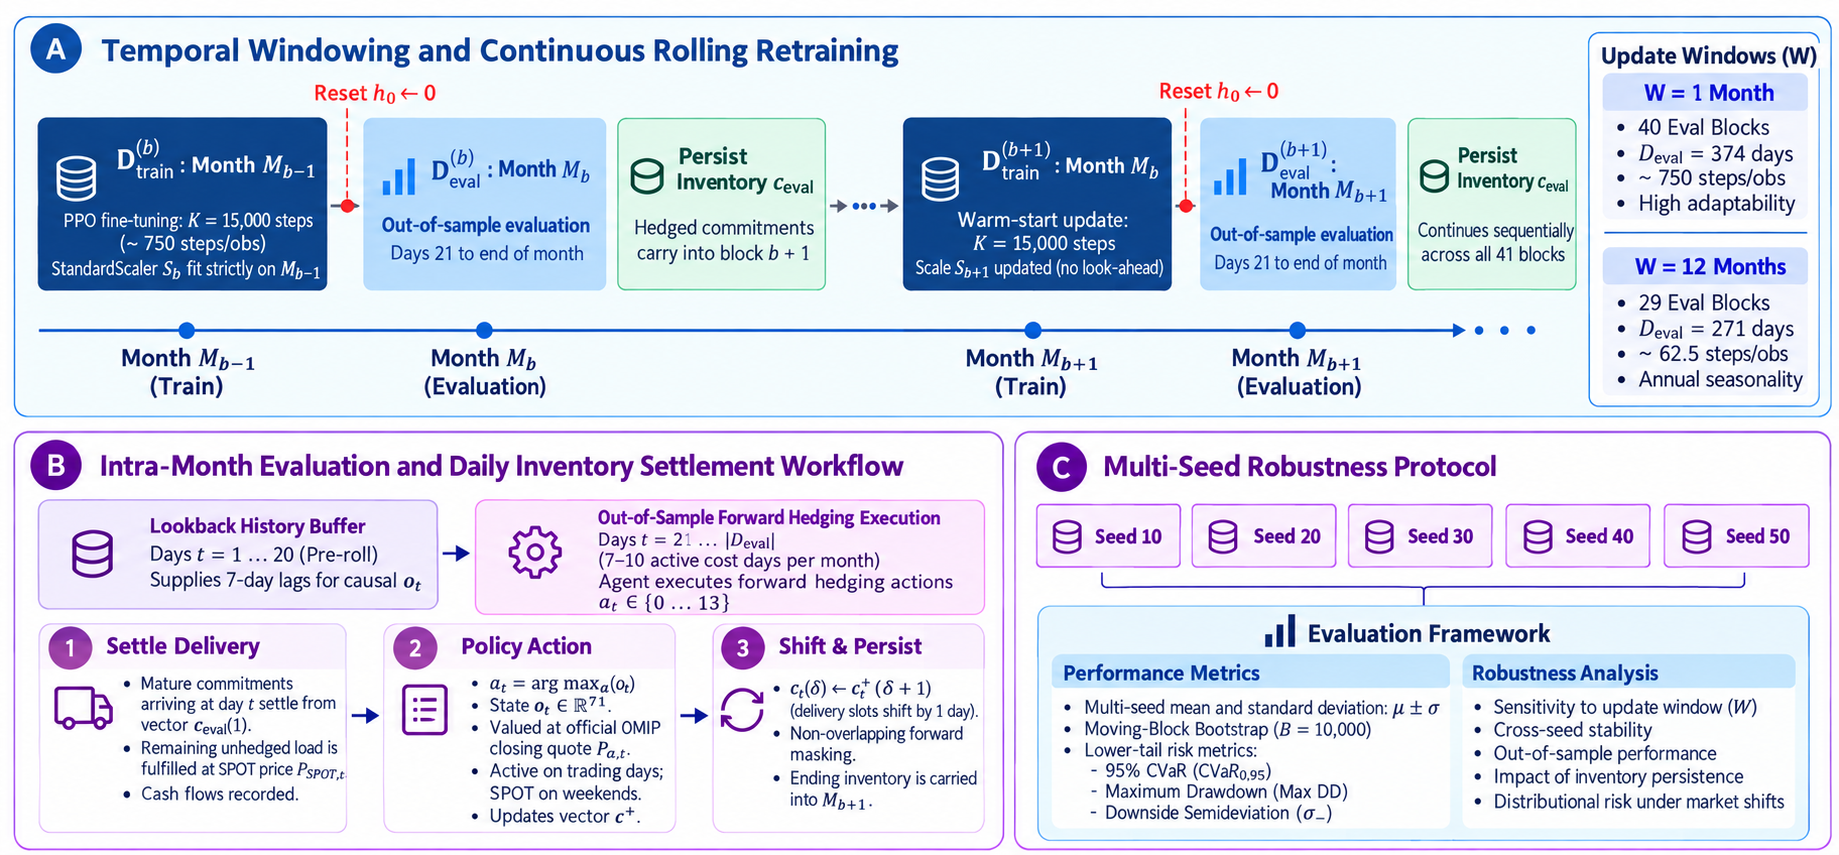
\includegraphics[width=\textwidth]{fig9_walk_forward_protocol.png}
    \caption{Continuous Walk-Forward rolling retraining protocol ($B=41$ calendar blocks, $B_{\text{eval}}=40$ evaluated blocks under $W=1$): (a) rolling window progression, (b) intra-month settlement workflow, and (c) multi-seed robustness evaluation framework. Conceptual layout design was assisted using Anthropic Claude 3.5 Sonnet to arrange workflow stages; all scientific logic, data, and final graphic rendering were programmed directly by the authors in Matplotlib.}
    \label{fig:walk_forward_protocol}
\end{figure*}

The choice of rolling update window $W$ ($W \in \{1, 3, 6, 12\}$ months) used in Algorithm~\ref{alg:walk_forward} to generate PPO rollouts ($K = 15{,}000$ steps) during each monthly retraining phase interacts directly with sample optimization intensity and temporal discounting. Because policy weights $\theta$ are updated via warm-start rather than re-initialized from scratch, $W$ governs the temporal recency of gradient updates while allowing the network to retain representations learned across preceding horizons. 

Importantly, holding total monthly interaction steps fixed at $K = 15{,}000$ across all window sizes introduces a methodological trade-off: a short window of $W = 1$ month ($N_W \approx 20$ active trading sessions) experiences approximately $K / N_W \approx 750$ environment steps per observation, $W=3$ months experiences $\approx 250$ steps/obs, $W=6$ months experiences $\approx 125$ steps/obs, whereas an annual window of $W = 12$ months ($N_W \approx 240$ sessions) experiences approximately $K / N_W \approx 62.5$ steps per observation. This fixed-$K$ protocol reflects a realistic operational deployment constraint where the monthly offline retraining computing budget is bounded. An alternative formulation would scale the training budget proportionally ($K(W) \propto N_W$, e.g., $K=180{,}000$ for $W=12$ to maintain 750 steps/obs); however, this would substantially increase computational runtime and risk overfitting to obsolete market regimes. Therefore, the empirical superiority of shorter windows reflects both greater data recency (mitigating non-stationarity) and higher optimization intensity per sample on recent regime dynamics.

Furthermore, setting the MDP discount factor to $\gamma = 0.99$ introduces an endogenous temporal discounting effect: cash flows realised at delivery offsets of 30, 90, and 180 days are discounted by $\gamma^{30} \approx 0.74$, $\gamma^{90} \approx 0.40$, and $\gamma^{180} \approx 0.16$, respectively. In combination with full-volume baseload commitments (locking 100\% of the load for all days in the contract window) and non-overlapping forward masking, this discounting structure naturally reinforces the policy's concentration on short-horizon products ($D_1$--$D_3$) over multi-month contracts ($M_1$--$M_6$).

At the start of each out-of-sample monthly evaluation block $b$, the persistent physical and financial inventory state $\mathbf{c}_{\text{eval}}$ (containing all active forward commitments locked in prior blocks that mature in month $b$ or beyond) is injected continuously into the evaluation environment, ensuring seamless temporal continuity of delivery commitments across retraining boundaries without artificial inventory liquidation. Simultaneously, the recurrent hidden state of the updated policy is cleanly re-initialized ($h_0 \leftarrow \mathbf{0}$, \texttt{episode\_starts = True}) to prevent latent vector misalignment under modified network weights $\theta$. The environment evaluates the out-of-sample days of each monthly block following an initial 20-step monthly feature history buffer ($D_{\text{eval}} = 374$ valid days across 40 blocks for $W=1$, $D_{\text{eval}} = 1{,}117$ days across 38 blocks for $W=3$, $D_{\text{eval}} = 1{,}029$ days across 35 blocks for $W=6$, and $D_{\text{eval}} = 271$ valid days across 29 blocks for $W=12$, with a strictly controlled common intersection of $N=271$ days). For reporting purposes, all reinforcement learning results represent the multi-seed mean across 5 independently trained seeds ($s \in \{10, 20, 30, 40, 50\}$) with across-seed standard deviation ($\pm \sigma$).

Finally, in Phase~4 (Exploratory Post-Selection Analysis), to determine the attainable performance ceiling of each architecture and state representation under matched optimization budgets, Bayesian hyperparameter optimisation is performed via Optuna \cite{akiba2019optuna} using the Tree-structured Parzen Estimator (TPE, seed $s=42$, 50 trials per architecture) on the primary hybrid configuration (\texttt{Dataset\_\allowbreak M8\_\allowbreak Physical\_\allowbreak NLP}, $W=1$ month). The optimal hyperparameter configuration identified for each architecture (RecurrentPPO LSTM and GTrXL Transformer) is subsequently frozen and transferred identically to evaluate the corresponding Quantitative Baseline (\texttt{Dataset\_\allowbreak Exogenous\_\allowbreak Commodities}) under single-environment execution ($n_{\text{envs}}=1$) across 5 independent random seeds (seeds 10--50). This matched transfer protocol enforces equal optimization budgets between state representations, although the architecture hyperparameters are naturally selected on the Hybrid feature space. The search space covers learning rate $\eta \in [10^{-5}, 10^{-3}]$ (log-uniform continuous), rollout buffer $n_{\text{steps}} \in [64, 256]$ (integer range sampled via uniform integer distribution), mini-batch size $\in [16, 128]$ (integer range), entropy coefficient $c_{\text{ent}} \in [0.005, 0.1]$ (log-uniform continuous), PPO clip range $\in [0.1, 0.3]$ (uniform continuous), and architectural parameters (LSTM hidden size $\in [64, 256]$ integer range for RecurrentPPO; feature extractor dimension $d_{\text{feat}} \in [64, 256]$ integer range and feedforward policy layers $[64, 64]$ for GTrXL). Because the Optuna objective evaluates savings over the 2023--2026 horizon (including 2026), Phase 4 is explicitly declared as an exploratory post-selection capacity analysis rather than an unbiased out-of-sample evaluation.

